\section{Planning} \label{section:plan}
The following plan contains the work parts (WP) of this graduation thesis and the expected breakdown of how long it would take to work on each of them. There are eight such WPs distributed over 32 weeks as follows : 
\begin{itemize}
    \item WP1	Literature study of gradient based XAI algorithms and overview of project
    \item WP2	Identifying datasets, metrics, optimizations required to build the pipeline
    \item WP3	Implementing the base framework, dataset loaders, metrics and optimisations
    \item WP4	Implementing the gradient based algorithms, Integrating Vision Transformers into the pipeline
    \item WP5	Perform Training, Experimentation with different modules, Hyper Parameter Optimization
    \item WP6	Testing and analysis
    \item WP7	Writing the report
    \item WP8	Preparing final presentation
\end{itemize}
\begin{figure}[!htbp]
  \centering
  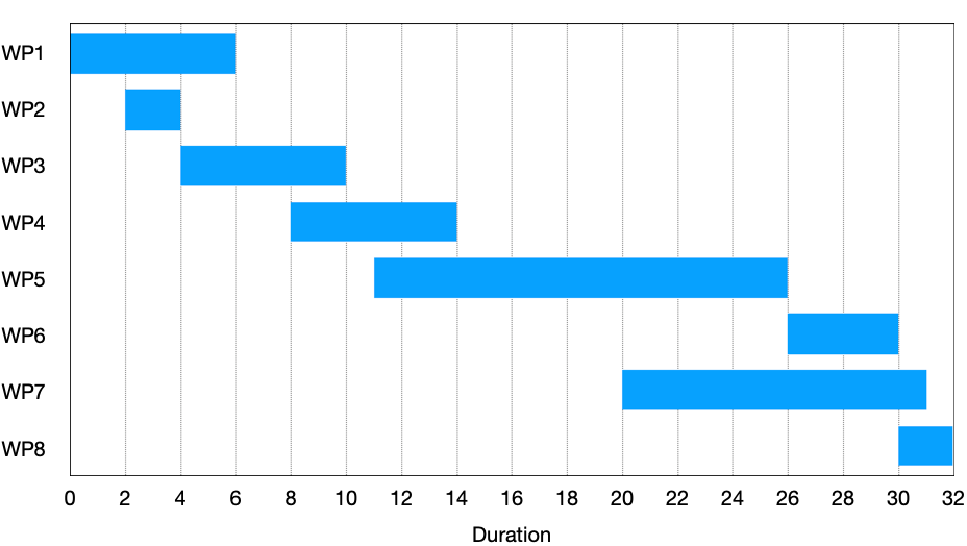
\includegraphics[width=.8\textwidth]{images/gantt_chart.pdf}
  \caption{Weekly Plan}
  \label{fig:plan}
\end{figure}

The timeline of the research is presented in this \hyperref[fig:plan]{Figure \ref{fig:plan}}.

\section{Resources and Support}
For the initial creation, testing and ideation of pipelines and network architecture,Wewill use my personal computer. It runs Linux and has a decent GPU. For the final testing of multiple architectures and models,Wewill make use of the Peregrine HPC Cluster's virtual NVIDIA Tesla v-100 nodes soWecan run batch experiments.\\
This work will be directly supervised by Dr. Hamidreza Kasaei. A co-supervisor is yet to be determined. The plan for meetings is to have a progress update every two weeks until completion. This schedule should remain stable for most of the project. There is no collaboration with any company so other related points do not apply here.